%% LyX 2.3.7 created this file.  For more info, see http://www.lyx.org/.
%% Do not edit unless you really know what you are doing.
\documentclass[journal,article,submit,pdftex,moreauthors]{mdpi}
\usepackage[utf8]{inputenc}
\usepackage{float}
\usepackage{url}
\usepackage{graphicx}

\makeatletter

%%%%%%%%%%%%%%%%%%%%%%%%%%%%%% LyX specific LaTeX commands.

\Title{Train neural networks with a hybrid method that incorporates a novel
simulated annealing procedure}

\TitleCitation{Train neural networks with a hybrid method that incorporates a novel
simulated annealing procedure}

\Author{Ioannis G. Tsoulos$^{1,*}$, Vasileios Charilogis$^{2}$ and Dimitrios
Tsalikakis$^{3}$}

\AuthorNames{Ioannis G. Tsoulos, Vasileios Charilogis and Dimitrios Tsalikakis }

\AuthorCitation{Tsoulos, I.G.; Charilogis, V.; Tsalikakis, D. }


\address{$^{1}$\quad{}Department of Informatics and Telecommunications,
University of Ioannina, Greece;itsoulos@uoi.gr\\
$^{2}$\quad{}Department of Informatics and Telecommunications, University
of Ioannina, Greece; v.charilog@uoi.gr\\
$^{3}\quad$Department of Engineering Informatics and Telecommunications,
University of Western Macedonia, 50100 Kozani, Greece;tsalikakis@gmail.com}


\corres{Correspondence: itsoulos@uoi.gr}


\abstract{In this paper, an innovative hybrid technique is proposed for the
efficient training of artificial neural networks, which are used both
in class learning problems and in data fitting problems. This hybrid
technique combines the well-tested technique of Genetic Algorithms
with an innovative variant of Simulated Annealing, in order to achieve
high learning rates for the neural networks. This variant was applied
periodically to randomly selected chromosomes from the population
of the Genetic Algorithm in order to reduce the training error achieved
by these chromosomes. The proposed method was tested on a wide series
of classification and data fitting problems from the relevant literature
and the results were compared against other methods. The comparison
with other neural network training techniques as well as the statistical
comparison revealed that the proposed method is significantly superior,
as it managed to significantly reduce the neural network training
error in the majority of the used datasets. }


\keyword{Artificial neural networks; Evolutionary techniques; Genetic algorithms;
Simulated Annealing }

\DeclareTextSymbolDefault{\textquotedbl}{T1}
%% Because html converters don't know tabularnewline
\providecommand{\tabularnewline}{\\}
\floatstyle{ruled}
\newfloat{algorithm}{tbp}{loa}
\providecommand{\algorithmname}{Algorithm}
\floatname{algorithm}{\protect\algorithmname}

%%%%%%%%%%%%%%%%%%%%%%%%%%%%%% User specified LaTeX commands.
%  LaTeX support: latex@mdpi.com 
%  For support, please attach all files needed for compiling as well as the log file, and specify your operating system, LaTeX version, and LaTeX editor.

%=================================================================


% For posting an early version of this manuscript as a preprint, you may use "preprints" as the journal and change "submit" to "accept". The document class line would be, e.g., \documentclass[preprints,article,accept,moreauthors,pdftex]{mdpi}. This is especially recommended for submission to arXiv, where line numbers should be removed before posting. For preprints.org, the editorial staff will make this change immediately prior to posting.

%--------------------
% Class Options:
%--------------------
%----------
% journal
%----------
% Choose between the following MDPI journals:
% acoustics, actuators, addictions, admsci, adolescents, aerospace, agriculture, agriengineering, agronomy, ai, algorithms, allergies, alloys, analytica, animals, antibiotics, antibodies, antioxidants, applbiosci, appliedchem, appliedmath, applmech, applmicrobiol, applnano, applsci, aquacj, architecture, arts, asc, asi, astronomy, atmosphere, atoms, audiolres, automation, axioms, bacteria, batteries, bdcc, behavsci, beverages, biochem, bioengineering, biologics, biology, biomass, biomechanics, biomed, biomedicines, biomedinformatics, biomimetics, biomolecules, biophysica, biosensors, biotech, birds, bloods, blsf, brainsci, breath, buildings, businesses, cancers, carbon, cardiogenetics, catalysts, cells, ceramics, challenges, chemengineering, chemistry, chemosensors, chemproc, children, chips, cimb, civileng, cleantechnol, climate, clinpract, clockssleep, cmd, coasts, coatings, colloids, colorants, commodities, compounds, computation, computers, condensedmatter, conservation, constrmater, cosmetics, covid, crops, cryptography, crystals, csmf, ctn, curroncol, currophthalmol, cyber, dairy, data, dentistry, dermato, dermatopathology, designs, diabetology, diagnostics, dietetics, digital, disabilities, diseases, diversity, dna, drones, dynamics, earth, ebj, ecologies, econometrics, economies, education, ejihpe, electricity, electrochem, electronicmat, electronics, encyclopedia, endocrines, energies, eng, engproc, ent, entomology, entropy, environments, environsciproc, epidemiologia, epigenomes, est, fermentation, fibers, fintech, fire, fishes, fluids, foods, forecasting, forensicsci, forests, foundations, fractalfract, fuels, futureinternet, futureparasites, futurepharmacol, futurephys, futuretransp, galaxies, games, gases, gastroent, gastrointestdisord, gels, genealogy, genes, geographies, geohazards, geomatics, geosciences, geotechnics, geriatrics, hazardousmatters, healthcare, hearts, hemato, heritage, highthroughput, histories, horticulturae, humanities, humans, hydrobiology, hydrogen, hydrology, hygiene, idr, ijerph, ijfs, ijgi, ijms, ijns, ijtm, ijtpp, immuno, informatics, information, infrastructures, inorganics, insects, instruments, inventions, iot, j, jal, jcdd, jcm, jcp, jcs, jdb, jeta, jfb, jfmk, jimaging, jintelligence, jlpea, jmmp, jmp, jmse, jne, jnt, jof, joitmc, jor, journalmedia, jox, jpm, jrfm, jsan, jtaer, jzbg, kidney, kidneydial, knowledge, land, languages, laws, life, liquids, literature, livers, logics, logistics, lubricants, lymphatics, machines, macromol, magnetism, magnetochemistry, make, marinedrugs, materials, materproc, mathematics, mca, measurements, medicina, medicines, medsci, membranes, merits, metabolites, metals, meteorology, methane, metrology, micro, microarrays, microbiolres, micromachines, microorganisms, microplastics, minerals, mining, modelling, molbank, molecules, mps, msf, mti, muscles, nanoenergyadv, nanomanufacturing, nanomaterials, ncrna, network, neuroglia, neurolint, neurosci, nitrogen, notspecified, nri, nursrep, nutraceuticals, nutrients, obesities, oceans, ohbm, onco, oncopathology, optics, oral, organics, organoids, osteology, oxygen, parasites, parasitologia, particles, pathogens, pathophysiology, pediatrrep, pharmaceuticals, pharmaceutics, pharmacoepidemiology, pharmacy, philosophies, photochem, photonics, phycology, physchem, physics, physiologia, plants, plasma, pollutants, polymers, polysaccharides, poultry, powders, preprints, proceedings, processes, prosthesis, proteomes, psf, psych, psychiatryint, psychoactives, publications, quantumrep, quaternary, qubs, radiation, reactions, recycling, regeneration, religions, remotesensing, reports, reprodmed, resources, rheumato, risks, robotics, ruminants, safety, sci, scipharm, seeds, sensors, separations, sexes, signals, sinusitis, skins, smartcities, sna, societies, socsci, software, soilsystems, solar, solids, sports, standards, stats, stresses, surfaces, surgeries, suschem, sustainability, symmetry, synbio, systems, taxonomy, technologies, telecom, test, textiles, thalassrep, thermo, tomography, tourismhosp, toxics, toxins, transplantology, transportation, traumacare, traumas, tropicalmed, universe, urbansci, uro, vaccines, vehicles, venereology, vetsci, vibration, viruses, vision, waste, water, wem, wevj, wind, women, world, youth, zoonoticdis 

%---------
% article
%---------
% The default type of manuscript is "article", but can be replaced by: 
% abstract, addendum, article, book, bookreview, briefreport, casereport, comment, commentary, communication, conferenceproceedings, correction, conferencereport, entry, expressionofconcern, extendedabstract, datadescriptor, editorial, essay, erratum, hypothesis, interestingimage, obituary, opinion, projectreport, reply, retraction, review, perspective, protocol, shortnote, studyprotocol, systematicreview, supfile, technicalnote, viewpoint, guidelines, registeredreport, tutorial
% supfile = supplementary materials

%----------
% submit
%----------
% The class option "submit" will be changed to "accept" by the Editorial Office when the paper is accepted. This will only make changes to the frontpage (e.g., the logo of the journal will get visible), the headings, and the copyright information. Also, line numbering will be removed. Journal info and pagination for accepted papers will also be assigned by the Editorial Office.

%------------------
% moreauthors
%------------------
% If there is only one author the class option oneauthor should be used. Otherwise use the class option moreauthors.

%---------
% pdftex
%---------
% The option pdftex is for use with pdfLaTeX. If eps figures are used, remove the option pdftex and use LaTeX and dvi2pdf.

%=================================================================
% MDPI internal commands - do not modify
\firstpage{1} 
 
\setcounter{page}{\@firstpage} 

\pubvolume{1}
\issuenum{1}
\articlenumber{0}
\pubyear{2024}
\copyrightyear{2024}
%\externaleditor{Academic Editor: Firstname Lastname} % For journal Automation, please change Academic Editor to "Communicated by"
\datereceived{}
\daterevised{ } % Comment out if no revised date
\dateaccepted{}
\datepublished{}
%\datecorrected{} % Corrected papers include a "Corrected: XXX" date in the original paper.
%\dateretracted{} % Corrected papers include a "Retracted: XXX" date in the original paper.
\hreflink{https://doi.org/} % If needed use \linebreak
%\doinum{}
%------------------------------------------------------------------
% The following line should be uncommented if the LaTeX file is uploaded to arXiv.org
%\pdfoutput=1

%=================================================================
% Add packages and commands here. The following packages are loaded in our class file: fontenc, inputenc, calc, indentfirst, fancyhdr, graphicx, epstopdf, lastpage, ifthen, lineno, float, amsmath, setspace, enumitem, mathpazo, booktabs, titlesec, etoolbox, tabto, xcolor, soul, multirow, microtype, tikz, totcount, changepage, attrib, upgreek, cleveref, amsthm, hyphenat, natbib, hyperref, footmisc, url, geometry, newfloat, caption

%=================================================================
%% Please use the following mathematics environments: Theorem, Lemma, Corollary, Proposition, Characterization, Property, Problem, Example, ExamplesandDefinitions, Hypothesis, Remark, Definition, Notation, Assumption
%% For proofs, please use the proof environment (the amsthm package is loaded by the MDPI class).

%=================================================================
% The fields PACS, MSC, and JEL may be left empty or commented out if not applicable
%\PACS{J0101}
%\MSC{}
%\JEL{}

%%%%%%%%%%%%%%%%%%%%%%%%%%%%%%%%%%%%%%%%%%
% Only for the journal Diversity
%\LSID{\url{http://}}

%%%%%%%%%%%%%%%%%%%%%%%%%%%%%%%%%%%%%%%%%%
% Only for the journal Applied Sciences:
%\featuredapplication{Authors are encouraged to provide a concise description of the specific application or a potential application of the work. This section is not mandatory.}
%%%%%%%%%%%%%%%%%%%%%%%%%%%%%%%%%%%%%%%%%%

%%%%%%%%%%%%%%%%%%%%%%%%%%%%%%%%%%%%%%%%%%
% Only for the journal Data:
%\dataset{DOI number or link to the deposited data set in cases where the data set is published or set to be published separately. If the data set is submitted and will be published as a supplement to this paper in the journal Data, this field will be filled by the editors of the journal. In this case, please make sure to submit the data set as a supplement when entering your manuscript into our manuscript editorial system.}

%\datasetlicense{license under which the data set is made available (CC0, CC-BY, CC-BY-SA, CC-BY-NC, etc.)}

%%%%%%%%%%%%%%%%%%%%%%%%%%%%%%%%%%%%%%%%%%
% Only for the journal Toxins
%\keycontribution{The breakthroughs or highlights of the manuscript. Authors can write one or two sentences to describe the most important part of the paper.}

%%%%%%%%%%%%%%%%%%%%%%%%%%%%%%%%%%%%%%%%%%
% Only for the journal Encyclopedia
%\encyclopediadef{Instead of the abstract}
%\entrylink{The Link to this entry published on the encyclopedia platform.}
%%%%%%%%%%%%%%%%%%%%%%%%%%%%%%%%%%%%%%%%%%

%%%%%%%%%%%%%%%%%%%%%%%%%%%%%%%%%%%%%%%%%%
% Only for the journal Advances in Respiratory Medicine
%\addhighlights{yes}
%\renewcommand{\addhighlights}{%

%\noindent This is an obligatory section in “Advances in Respiratory Medicine”, whose goal is to increase the discoverability and readability of the article via search engines and other scholars. Highlights should not be a copy of the abstract, but a simple text allowing the reader to quickly and simplified find out what the article is about and what can be cited from it. Each of these parts should be devoted up to 2~bullet points.\vspace{3pt}\\
%\textbf{What are the main findings?}
% \begin{itemize}[labelsep=2.5mm,topsep=-3pt]
% \item First bullet.
% \item Second bullet.
% \end{itemize}\vspace{3pt}
%\textbf{What is the implication of the main finding?}
% \begin{itemize}[labelsep=2.5mm,topsep=-3pt]
% \item First bullet.
% \item Second bullet.
% \end{itemize}
%}
%%%%%%%%%%%%%%%%%%%%%%%%%%%%%%%%%%%%%%%%%%

\makeatother

\begin{document}
\maketitle

\section{Introduction}

Artificial Neural networks (ANNs) \citep{nn1,nn2} are widely used
parametric tools, where a series of methods have been developed to
identify the optimal set of these parameters, commonly called weights
or processing units. ANNs have been used in a variety of scientific
problems, such as problems from physics \citep{nnphysics1,nnphysics2,nnphysics3},
chemistry \citep{nnchem1,nnchem2,nnchem3}, economics \citep{nnecon1,nnecon2,nncecon3},
medicine \citep{nnmed1,nnmed2} etc. Furthermore, in recent years,
neural networks have been incorporated into a variety of practical
problems, such as flood simulation \citep{nn_flood}, solar radiation
prediction \citep{nn_solar}, agricultural problems \citep{nn_agro},
solution of problems in wireless communications \citep{nn_wireless}
etc.

Commonly, a neural network is expressed as function $N(\overrightarrow{x},\overrightarrow{w})$,
where the vector $\overrightarrow{x}$ expresses the input pattern
and the vector $\overrightarrow{w}$ represents the weight vector
of the neural network. The methods aimed at training the artificial
neural network deal with the efficient adjustment of the weight vector
$\overrightarrow{w}$ to minimize the training error defined as: 

\begin{equation}
E\left(N\left(\overrightarrow{x},\overrightarrow{w}\right)\right)=\sum_{i=1}^{M}\left(N\left(\overrightarrow{x}_{i},\overrightarrow{w}\right)-y_{i}\right)^{2}\label{eq:eq1}
\end{equation}
The set set $\left(\overrightarrow{x_{i}},y_{i}\right),\ i=1,...,M$
defines the train set for the neural network, where the value $y_{i}$
represent the the actual output for pattern $\overrightarrow{x_{i}}$
. Neural networks can be expressed also in close analytic form, as
show in \citep{nnc}. As it was shown any neural network can be expressed
as function
\begin{equation}
N\left(\overrightarrow{x},\overrightarrow{w}\right)=\sum_{i=1}^{H}w_{(d+2)i-(d+1)}\sigma\left(\sum_{j=1}^{d}x_{j}w_{(d+2)i-(d+1)+j}+w_{(d+2)i}\right)\label{eq:nn}
\end{equation}
The parameter $H$ defines the number of processing units and the
constant $d$ represents the dimension of pattern $\overrightarrow{x}$.
The function $\sigma(x)$ is called sigmoid function, and it is defined
as: 
\begin{equation}
\sigma(x)=\frac{1}{1+\exp(-x)}\label{eq:sig}
\end{equation}
The number of elements in the weight vector are calculated as: $n=(d+2)H$. 

In the recent bibliography, a series of methods have been proposed
to minimize the equation \ref{eq:eq1}, such as the Back Propagation
method \citep{bpnn,bpnn2}, the Levenberg-Marquardt method \citep{nn_leve},
the RPROP method \citep{rpropnn,rpropnn3,rpropnn2}, Quasi Newton
methods \citep{quasinn,quasinn2}, Particle Swarm Optimization \citep{psonn,psonn2},
the Differential Evolution method \citep{nn_de}, etc. A survey of
stochastic methods for training neural networks can be found in the
work of Zhang and Suganthan \citep{nn_survey}.

Due to the wide application of artificial neural networks in various
fields, but also due to the difficulties faced by traditional optimization
techniques in minimizing the training error, a series of hybrid techniques
have been developed to more effectively reduce this error. Among these
methods there is the method of\textbf{ }Yaghini et al. \citep{nnhybrid1}
that combines Particle Swarm Optimization and the Back Propagation
technique. Also, Chen at al \citep{nnhybrid2} has proposed a hybrid
method that incorporates particle swarm optimization and Cuckoo Search
\citep{csmethod}.

Another important issue of neural networks that has been thoroughly
studied in the recent literature is the initialization of the weights
for the network. The methods developed for the initialization issue
include utilization of decision trees\textbf{ }\citep{nninit1}, an
initialization technique based on the Cauchy's inequality \citep{weight_init2},
discriminant learning \citep{weight_init3} etc. A recent paper by
Narkhede et al. \citep{nninitreview} presents various techniques
for the initialization of the weights.

Due to the complexity of the training techniques but also due to the
fact that the number of required parameters increases with the increase
in the dimension of the problem, a number of training techniques have
been developed that take advantage of modern parallel computing structures.
For example, there are implementations of neural networks on GPU cards
\citep{nn_gpu1}, incorporation of GPU programming techniques on neural
network training for face recognition \citep{nn_gpu2}, molecular
dynamics simulation using neural networks that are executed on GPU
cards \citep{nn_gpu3} etc. A comparative study of GPU programming
models used for neural network training can be found in the work of
Pallipuram et al \citep{nn_gpu_review}.

In this work, the use of a hybrid optimization technique is proposed
for the training of artificial neural networks. In this hybrid technique,
Genetic Algorithms are used as a basic technique for training neural
networks. Genetic algorithms, which were initially suggested by John
Holland \citep{Holland}, are inspired by biology, and are form trial
solutions of any optimization problem. These solutions are improved
gradually by a process that mimics natural evolution, such as mutation,
natural selection, and crossover \citep{Stender,Goldberg,Michaelewicz}.
Genetic algorithms have proven their efficiency, and they have been
applied on a wide series of problems, such as networking \citep{ga_problem1},
robotics \citep{ga_problem2,ga_problem3}, energy problems \citep{ga_problem4,ga_problem5}
etc. Although Genetic Algorithms can satisfactorily train an artificial
neural network, in many cases they get trapped in local minimum of
the training error and this results in poor performance of the neural
network when applied to the test set. To improve the performance of
genetic algorithms, it is proposed to periodically apply a minimization
technique to randomly selected chromosomes of the genetic population.
This minimization method that is applied here, is a modified version
of the Simulated Annealing method \citep{siman_main}. Simulated annealing
has been applied in many cases, such as police district design \citep{siman_problem1},
portfolio problems \citep{siman_problem2}, energy problems \citep{siman_problem3}
etc. The new method was tested on a wide series of classification
and regression problems, and it was compared against other optimization
methods. From the experimental comparison of the results, it appears
that the proposed technique significantly improves the performance
of genetic algorithms in the training of artificial neural networks.

The rest of this article is divided as follows: in section \ref{sec:Materials-and-Methods}
the proposed method is discussed in detail. In section \ref{sec:Results}
the used datasets are presented as well as the experimental results,
and finally, in section \ref{sec:Conclusions} the results are discussed
thoroughly and some guidelines for future research are provided.

\section{The proposed method\label{sec:Materials-and-Methods}}

The new Simulated Annealing variant is described in this section,
as well as the overall algorithm, that will be used to train artificial
neural networks for classification and regression problems.

\subsection{The new Simulated Annealing variant \label{subsec:The-new-Simulated}}

A new variant of the Simulated Annealing method is utilized as a local
search procedure in the Genetic Algorithm. This method has been applied
to many problems and is distinguished for its adaptability but also
for the ability to aim for lower values of the objective function,
especially if combined with intelligent techniques to reduce the temperature
factor. In the proposed modification of the method, the optimization
procedure initiates from the current state of a chromosome and by
applying stochastic techniques a search is made for nearby representations
with lower values of the error function. The steps of the proposed
method are illustrated in Algorithm\textbf{ }\ref{alg:siman}.

\textbf{}
\begin{algorithm}[H]
\textbf{\caption{The used variant of the Simulated Annealing algorithm.\label{alg:siman}}
}

\textbf{procedure }siman\textbf{$\left(x_{0}\right)$}
\begin{enumerate}
\item \textbf{Set $k=0$, $T_{0}>0,\ \epsilon>0,$$r_{T}>0,\ r_{T}<1$}.\textbf{
}The parameter $T_{0}$ defines the initial temperature of the algorithm.
\item \textbf{Set }$N_{eps}>0$, a positive integer number. This number
defines the number of samples that will be created in every iteration.
\item \textbf{Set }the parameter $F\in[0,1]$. This value specifies the
range of changes that can be made to an element of a chromosome, as
a percentage of its original value. 
\item \textbf{Set} the positive integer parameter $N_{R}$. This parameter
indicates the number of possible random changes in the chromosome.
\item \textbf{Set $x_{b}=x_{0},f_{b}=f\left(x_{b}\right)$.}
\item \textbf{For $i=1\ldots N_{\mbox{eps}}$ \label{enu:For-}}

\begin{enumerate}
\item \textbf{Set $x^{t}=x_{k}$ }as a candidate point.
\item \textbf{For $j=1\ldots N_{R}$}
\begin{enumerate}
\item \textbf{Set $p=\mbox{rand}\left(1,\mbox{size}\left(x^{t}\right)\right)$},
a randomly selected position in the chromosome.
\item \textbf{Set $x_{p}^{t}=x_{p}^{t}+\mbox{rand}\left(-F,F\right)x_{p}^{t}$}
\end{enumerate}
\item \textbf{EndFor}
\item \textbf{If $f\left(x^{t}\right)\le f\left(x_{k}\right)$ then $x_{k+1}=x^{t}$}
\item \textbf{Else Set $x_{k+1}=x^{t}$ }with probability\textbf{ $\min\left\{ 1,\exp\left(-\frac{f\left(x^{t}\right)-f\left(x_{k}\right)}{T_{k}}\right)\right\} $}
\item \textbf{If $f\left(x^{t}\right)<f_{b}$ then $x_{b}=x^{t},f_{b}=f\left(x^{t}\right)$.}
\end{enumerate}
\item \textbf{EndFor}
\item \textbf{Set $T_{k+1}=T_{k}r_{T}$}
\item \textbf{Set $k=k+1$.}
\item \textbf{If $T_{k}\le\epsilon$ stop.}
\item \textbf{Goto step \ref{enu:For-}.}
\item \textbf{Return $x_{b}$}
\end{enumerate}
\textbf{end }siman
\end{algorithm}
The method initiates from chromosome $x_{0}$ and in every iteration
and it produces random points near to the original chromosome. The
integer parameter $N_{R}$ defines the number of changes that will
be made in the chromosome and the double precision parameter $F$
controls the magnitude of changes. The algorithm starts from high
values of the temperature $T_{0}$, which is linearly decreased in
each iteration. At high temperatures, the algorithm more readily accepts
values that it can with higher function values to more efficiently
explore the search space, but at lower values the algorithm focuses
on improving the best function value it has discovered.

\subsection{The overall algorithm}

A genetic algorithm is used as the base algorithm for neural network
training. Genetic algorithms have been used also in the recent bibliography
for neural network training in various cases, such as for drug design
\citep{ga_drug}, gear fault detection \citep{ga_gear}, forecasting
models \citep{ga_forecasting} etc. The genetic algorithm is enhanced
by the addition of a periodical application of the new Simulated Annealing
variant, described in the previous subsection. The main steps of the
overall algorithm are listed below.
\begin{enumerate}
\item \textbf{Initialization Step}
\begin{enumerate}
\item \textbf{Define }as $N_{c}$ the number of chromosomes and as $N_{g}$
the maximum number of generations. 
\item \textbf{Define }the selection rate $p_{s}$ and the mutation rate
$p_{m}$ with $p_{s}\in[0,1]$ and $p_{m}\in[0,1]$.
\item \textbf{Set }as\textbf{ $N_{I}$} the number of generations passed
before the modified Simulated Algorithm will be applied.
\item \textbf{Set }as\textbf{ $N_{K}$ }the number of chromosomes that will
be altered by the modified Simulated Annealing algorithm.
\item \textbf{Perform }a random initialization of the $N_{c}$ chromosomes.
Each chromosome represents a different set of randomly initialized
weights for the neural network.
\item \textbf{Set} $k=0$.
\end{enumerate}
\item \textbf{For} each chromosome\textbf{ }$g_{i},\ i=1,\ldots,N_{c}$ 
\begin{enumerate}
\item \textbf{Formulate }a neural network\textbf{ $N(\overrightarrow{x},\overrightarrow{g_{i}})$}
\item \textbf{Calculate} the fitness $f_{i}=\sum_{j=1}^{M}\left(N\left(\overrightarrow{x}_{j},\overrightarrow{g_{i}}\right)-y_{j}\right)^{2}$
of chromosome $g_{i}$ and for the given dataset.\textbf{\label{enu:Fitness-calculation-Step}}
\end{enumerate}
\item \textbf{Genetic operations step}
\begin{enumerate}
\item \textbf{Selection procedure.} The chromosomes are sorted with respect
to the associated fitness values. The first $\left(1-p_{s}\right)\times N_{c}$
chromosomes having the lowest fitness values are copied to the next
generation. The rest of the chromosomes are replaced by offspings
produced in the crossover procedure. 
\item \textbf{Crossover procedure}: In the crossover procedure pairs of
chromosomes are selected from the population using tournament selection.
For each pair $(z,w)$ of selected parents two new chromosomes $\tilde{z}$
and $\tilde{w}$ are formulated using the following scheme
\begin{eqnarray}
\tilde{z_{i}} & = & a_{i}z_{i}+\left(1-a_{i}\right)w_{i}\nonumber \\
\tilde{w_{i}} & = & a_{i}w_{i}+\left(1-a_{i}\right)z_{i}\label{eq:crossover_ali-1}
\end{eqnarray}
where $i=1,\ldots,n$. The randomly selected values $a_{i}$ are chosen
in the range $[-0.5,1.5]$ \citep{kaelo}. 
\item \textbf{Mutation procedure}:\textbf{ }
\begin{enumerate}
\item \textbf{For} each chromosome $g_{i},\ i=1,\ldots,N_{c}$ do
\begin{enumerate}
\item \textbf{For} every element $\ j=1,\ldots,n$ of $g_{i}$ a random
number $r\in\left[0,1\right]$ is produced. The corresponding element
is altered randomly if $r\le p_{m}$.
\end{enumerate}
\item \textbf{EndFor} 
\end{enumerate}
\end{enumerate}
\item \textbf{Local method step}
\begin{enumerate}
\item \textbf{If} $k\ \mbox{mod}\ N_{I}=0$ \textbf{then}
\begin{enumerate}
\item \textbf{For} $i=1,\ldots,N_{K}$ do
\begin{enumerate}
\item \textbf{Select} a random chromosome $g^{r}$
\item \textbf{Apply} the siman algorithm: $g^{r}=\mbox{siman}\left(g^{r}\right)$
of subsection \ref{subsec:The-new-Simulated}.
\end{enumerate}
\item \textbf{EndFo}r
\end{enumerate}
\item \textbf{Endif}
\end{enumerate}
\item \textbf{Termination Check Step}
\begin{enumerate}
\item \textbf{Set} $k=k+1$ 
\item \textbf{If} $k\ge N_{g}$ then goto \textbf{Termination} Step, else
goto \ref{enu:Fitness-calculation-Step}.
\end{enumerate}
\item \textbf{Termination step }
\begin{enumerate}
\item \textbf{Denote }as\textbf{ $g^{*}$ }the chromosome with the lowest
fitness value.
\item \textbf{Formulate }the neural network\textbf{ $N(\overrightarrow{x},\overrightarrow{g^{*}})$}
\item \textbf{Apply} a local search procedure to $g^{*}$. The local search
method used in the current work is a BFGS variant of Powell \citep{Powell}.
\item \textbf{Apply} the neural network \textbf{$N(\overrightarrow{x},\overrightarrow{g^{*}})$
}on the test of the objective problem and report the result.
\end{enumerate}
\end{enumerate}

\section{Results\label{sec:Results}}

The proposed work was tested on a series of well - known classification
and regression datasets from the recent bibliography and it was compared
other optimization methods, used to train neural networks. The used
datasets can be obtained freely from the following websites:
\begin{enumerate}
\item The UCI dataset repository, \url{https://archive.ics.uci.edu/ml/index.php}(accessed
on 18 June 2024)\citep{UCL}
\item The Keel repository, \url{https://sci2s.ugr.es/keel/datasets.php}(accessed
on 18 June 2024)\citep{Keel}.
\item The Statlib URL \url{http://lib.stat.cmu.edu/datasets/ }(accessed
on 18 June 2024). 
\end{enumerate}

\subsection{Classification datasets }

A series of classification datasets were used in the conducted experiments.
Their description has as follows:
\begin{enumerate}
\item \textbf{Appendictis} a medical dataset, suggested in \citep{appendicitis}. 
\item \textbf{Australian} dataset \citep{australian}, used in credit card
transactions.
\item \textbf{Bands} dataset, used to detect printing problems.
\item \textbf{Balance} dataset \citep{balance}, which is related to some
psychological experiments.
\item \textbf{Circular} dataset, which is an artificial dataset.
\item \textbf{Cleveland} dataset, a medical dataset \citep{cleveland1,cleveland2}.
\item \textbf{Dermatology} dataset \citep{dermatology}, which is a dataset
related to dermatological deceases. 
\item \textbf{Ecoli} dataset, a dataset about protein localization sites
of proteins\citep{ecoli}.
\item \textbf{Fert }dataset. Fertility dataset related to relation of sperm
concentration and demographic data.
\item \textbf{Heart} dataset \citep{heart}, a medical dataset used to detect
heart diseases.
\item \textbf{HeartAttack} dataset, used to predict heart attacks. 
\item \textbf{HouseVotes} dataset \citep{housevotes}, related to votes
in the U.S. House of Representatives. 
\item \textbf{Liverdisorder} dataset \citep{liver}, used to detect liver
disorders.
\item \textbf{Parkinsons} dataset, used to detect the Parkinson's disease
(PD)\citep{parkinsons}.
\item \textbf{Pima} dataset \citep{pima}, a medical dataset used to detect
the presence of diabetes.
\item \textbf{Popfailures} dataset \citep{popfailures}, a dataset related
to climate measurements.
\item \textbf{Regions2} dataset, related to hepatitis C \citep{regions}. 
\item \textbf{Saheart} dataset \citep{saheart}, used to detect heart diseases.
\item \textbf{Segment} dataset \citep{segment}, used in image processing
tasks.
\item \textbf{Sonar} dataset \citep{sonar}, used to discriminate sonar
signals.
\item \textbf{Spiral} dataset, an artificial dataset.
\item \textbf{Wdbc} dataset \citep{wdbc}, a medical dataset used to detect
cancer..
\item \textbf{Wine} dataset, used to detect the quality of wines. \citep{wine1,wine2}.
\item \textbf{Eeg} datasets, a dataset related to EEG measurements \citep{eeg}
and the following cases were used: Z\_F\_S, ZO\_NF\_S and ZONF\_S.
\item \textbf{Zoo} dataset \citep{zoo}, used to classify animals in seven
predefined categories.
\end{enumerate}

\subsection{Regression datasets }

The description of the used regression datasets has as follows:
\begin{enumerate}
\item \textbf{Airfoil }dataset, a dataset provided by NASA \citep{airfoil}.
\item \textbf{BK} dataset \citep{Stat}, used for points prediction in a
basketball game. 
\item \textbf{BL} dataset, it contains measurements from an experiment related
to electricity.
\item \textbf{Baseball} dataset, used to calculate the income of baseball
players. 
\item \textbf{Dee} dataset, used to calculate the price of electricity.
\item \textbf{EU, }downloaded from the STALIB repository.
\item \textbf{FY, }This dataset measures the longevity of fruit flies. 
\item \textbf{HO} dataset, downloaded from the STALIB repository.
\item \textbf{Housing} dataset, mentioned in \citep{housing}.
\item \textbf{LW} dataset, related to risk factors associated with low weight
babies.
\item \textbf{MORTGAGE} dataset, related to economic data from USA.
\item \textbf{MUNDIAL, }provided from the STALIB repository.
\item \textbf{PL} dataset, provided from the STALIB repository.
\item \textbf{QUAKE} dataset, that is used to measure the strength of a
earthquake.
\item \textbf{REALESTATE, }provided from the STALIB repository.
\item \textbf{SN} dataset. It contains measurements from an experiment related
to trellising and pruning. 
\item \textbf{Treasury} dataset, related to economic data from USA.
\item \textbf{VE} dataset, provided from the STALIB repository.
\end{enumerate}

\subsection{Experimental results}

A series of experiments were conducted to test the efficiency of the
used method as well as its stability. The experiments were conducted
using the freely available optimization environment of Optimus, that
can be downloaded from \url{https://github.com/itsoulos/GlobalOptimus/}(
accessed on 18 June 2024 ). The experiments were conducted 30 times
using different seeds for the random generator each time. The experiments
were validated using the method of 10 - fold cross validation. The
average classification error is reported for the classification datasets
and the average regression error is shown for the regression error.
The errors are reported on the test set. The experiments were executed
on a system equipped with an AMD Ryzen 5950X processor, 128GB of RAM.
The used operating system was the Debian Linux operating system. The
values of the parameters for all used algorithms are shown in Table
\ref{tab:settings}.

\begin{table}[H]
\caption{Values for the experimental parameters.\label{tab:settings}}

\centering{}%
\begin{tabular}{|c|c|}
\hline 
PARAMETER & VALUE\tabularnewline
\hline 
\hline 
$N_{c}$ & 500\tabularnewline
\hline 
$N_{g}$ & 200\tabularnewline
\hline 
$L_{I}$ & 20\tabularnewline
\hline 
$L_{K}$ & 20\tabularnewline
\hline 
$p_{s}$ & 0.10\tabularnewline
\hline 
$p_{m}$ & 0.05\tabularnewline
\hline 
$H$ & 10\tabularnewline
\hline 
$F$ & 0.10\tabularnewline
\hline 
$N_{R}$ & 20\tabularnewline
\hline 
\end{tabular}
\end{table}
The comparative results for the classification datasets are listed
in Table \ref{tab:expClass} and the results for the regression datasets
are shown in Table \ref{tab:expRegression}. The following applies
to all tables with experimental results:
\begin{enumerate}
\item The column DATASET denotes the name of the used dataset.
\item The column BFGS denotes the application of the BFGS optimization method
to train a neural network with $H$ processing nodes.
\item The column PSO denotes the application of a Particle Swarm Optimizer
with $N_{c}$ particles to train a neural network with $H$ processing
nodes.
\item The column GENETIC stands for the application of a Genetic Algorithm
with the parameters shown in Table \ref{tab:settings} to train a
neural network with $H$ processing nodes.
\item The column PROPOSED denotes the application of the proposed method
with the parameters of Table \ref{tab:settings} on a neural network
with $H$ hidden nodes.
\item The row AVERAGE denotes the average classification or regression error
for all datasets.
\end{enumerate}
\begin{table}[H]
\caption{Experimental results using a series of optimization methods for the
classification datasets. Numbers in cells denote average classification
error as measured on the test set.\label{tab:expClass}}

\centering{}%
\begin{tabular}{|c|c|c|c|c|}
\hline 
\textbf{DATASET} & \textbf{BFGS} & \textbf{PSO} & \textbf{GENETIC} & \textbf{PROPOSED}\tabularnewline
\hline 
\hline 
APPENDICITIS & 18.00\% & 25.00\% & 24.40\% & 22.60\%\tabularnewline
\hline 
AUSTRALIAN & 38.13\% & 38.30\% & 36.64\% & 32.42\%\tabularnewline
\hline 
BALANCE & 8.64\% & 7.97\% & 8.36\% & 8.10\%\tabularnewline
\hline 
BANDS & 36.67\% & 36.61\% & 34.92\% & 34.53\%\tabularnewline
\hline 
CIRCULAR & 6.08\% & 4.24\% & 5.13\% & 4.35\%\tabularnewline
\hline 
CLEVELAND & 77.55\% & 62.31\% & 57.21\% & 42.62\%\tabularnewline
\hline 
DERMATOLOGY & 52.92\% & 17.69\% & 16.60\% & 12.12\%\tabularnewline
\hline 
ECOLI & 69.52\% & 61.30\% & 54.67\% & 47.18\%\tabularnewline
\hline 
FERT & 23.20\% & 24.00\% & 28.50\% & 25.20\%\tabularnewline
\hline 
HEART & 39.44\% & 34.67\% & 26.41\% & 16.59\%\tabularnewline
\hline 
HEARTATTACK & 46.67\% & 37.83\% & 29.03\% & 20.13\%\tabularnewline
\hline 
HOUSEVOTES & 7.13\% & 7.87\% & 7.00\% & 7.13\%\tabularnewline
\hline 
LIVERDISORDER & 42.59\% & 39.82\% & 37.09\% & 32.88\%\tabularnewline
\hline 
PARKINSONS & 27.58\% & 23.58\% & 16.58\% & 16.63\%\tabularnewline
\hline 
PIMA & 35.59\% & 35.17\% & 34.21\% & 30.08\%\tabularnewline
\hline 
POPFAILURES & 5.24\% & 7.80\% & 4.17\% & 5.44\%\tabularnewline
\hline 
REGIONS2 & 36.28\% & 31.43\% & 33.53\% & 27.69\%\tabularnewline
\hline 
SAHEART & 37.48\% & 34.80\% & 34.85\% & 34.56\%\tabularnewline
\hline 
SEGMENT & 68.97\% & 53.88\% & 46.30\% & 28.41\%\tabularnewline
\hline 
SONAR & 25.85\% & 24.70\% & 22.40\% & 19.80\%\tabularnewline
\hline 
SPIRAL & 47.99\% & 46.31\% & 47.67\% & 44.54\%\tabularnewline
\hline 
WDBC & 29.91\% & 9.98\% & 7.87\% & 5.66\%\tabularnewline
\hline 
WINE & 59.71\% & 32.71\% & 22.88\% & 10.59\%\tabularnewline
\hline 
Z\_F\_S & 39.37\% & 38.73\% & 24.60\% & 11.10\%\tabularnewline
\hline 
ZO\_NF\_S & 43.04\% & 30.38\% & 21.54\% & 6.86\%\tabularnewline
\hline 
ZONF\_S & 15.62\% & 6.92\% & 4.36\% & 2.48\%\tabularnewline
\hline 
ZOO & 10.70\% & 9.20\% & 9.50\% & 7.60\%\tabularnewline
\hline 
\textbf{AVERAGE} & \textbf{35.18\%} & \textbf{29.01\%} & \textbf{25.79\%} & \textbf{20.64\%}\tabularnewline
\hline 
\end{tabular}
\end{table}

\begin{table}[H]
\begin{centering}
\caption{Experimental results for different optimization methods on a series
of regression datasets. Numbers in cells denote average regression
error as measure on the test set.\label{tab:expRegression}}
\begin{tabular}{|c|c|c|c|c|}
\hline 
\textbf{DATASET} & \textbf{BFGS} & \textbf{PSO} & \textbf{GENETIC} & \textbf{PROPOSED}\tabularnewline
\hline 
\hline 
AIRFOIL & 0.003 & 0.001 & 0.001 & 0.001\tabularnewline
\hline 
BK & 0.36 & 0.33 & 0.26 & 0.18\tabularnewline
\hline 
BL & 1.09 & 2.49 & 2.23 & 0.42\tabularnewline
\hline 
BASEBALL & 119.63 & 82.81 & 64.60 & 57.47\tabularnewline
\hline 
DEE & 2.36 & 0.43 & 0.47 & 0.23\tabularnewline
\hline 
EU & 607.61 & 407.35 & 252.97 & 216.65\tabularnewline
\hline 
FY & 0.19 & 0.05 & 0.65 & 0.23\tabularnewline
\hline 
HO & 0.62 & 0.03 & 0.37 & 0.06\tabularnewline
\hline 
HOUSING & 97.38 & 43.28 & 35.97 & 23.77\tabularnewline
\hline 
LW & 0.26 & 0.03 & 0.54 & 0.27\tabularnewline
\hline 
MORTGAGE & 8.23 & 1.47 & 0.40 & 0.05\tabularnewline
\hline 
MUNDIAL & 0.05 & 0.08 & 1.22 & 0.28\tabularnewline
\hline 
PL & 0.11 & 0.06 & 0.03 & 0.02\tabularnewline
\hline 
QUAKE & 0.09 & 0.06 & 0.12 & 0.06\tabularnewline
\hline 
REALESTATE & 128.94 & 81.41 & 81.19 & 72.95\tabularnewline
\hline 
SN & 0.16 & 0.40 & 0.20 & 0.05\tabularnewline
\hline 
TREASURY & 9.91 & 2.32 & 0.44 & 0.26\tabularnewline
\hline 
VE & 1.92 & 0.32 & 2.43 & 1.63\tabularnewline
\hline 
\textbf{AVERAGE} & \textbf{54.38} & \textbf{34.61} & \textbf{24.67} & \textbf{20.81}\tabularnewline
\hline 
\end{tabular}
\par\end{centering}
\end{table}
The statistical comparison between the used methods for the classification
datasets is shown in Figure \ref{fig:statClass}, while for the regression
datasets in Figure \ref{fig:statRegression}. 

\begin{figure}[H]
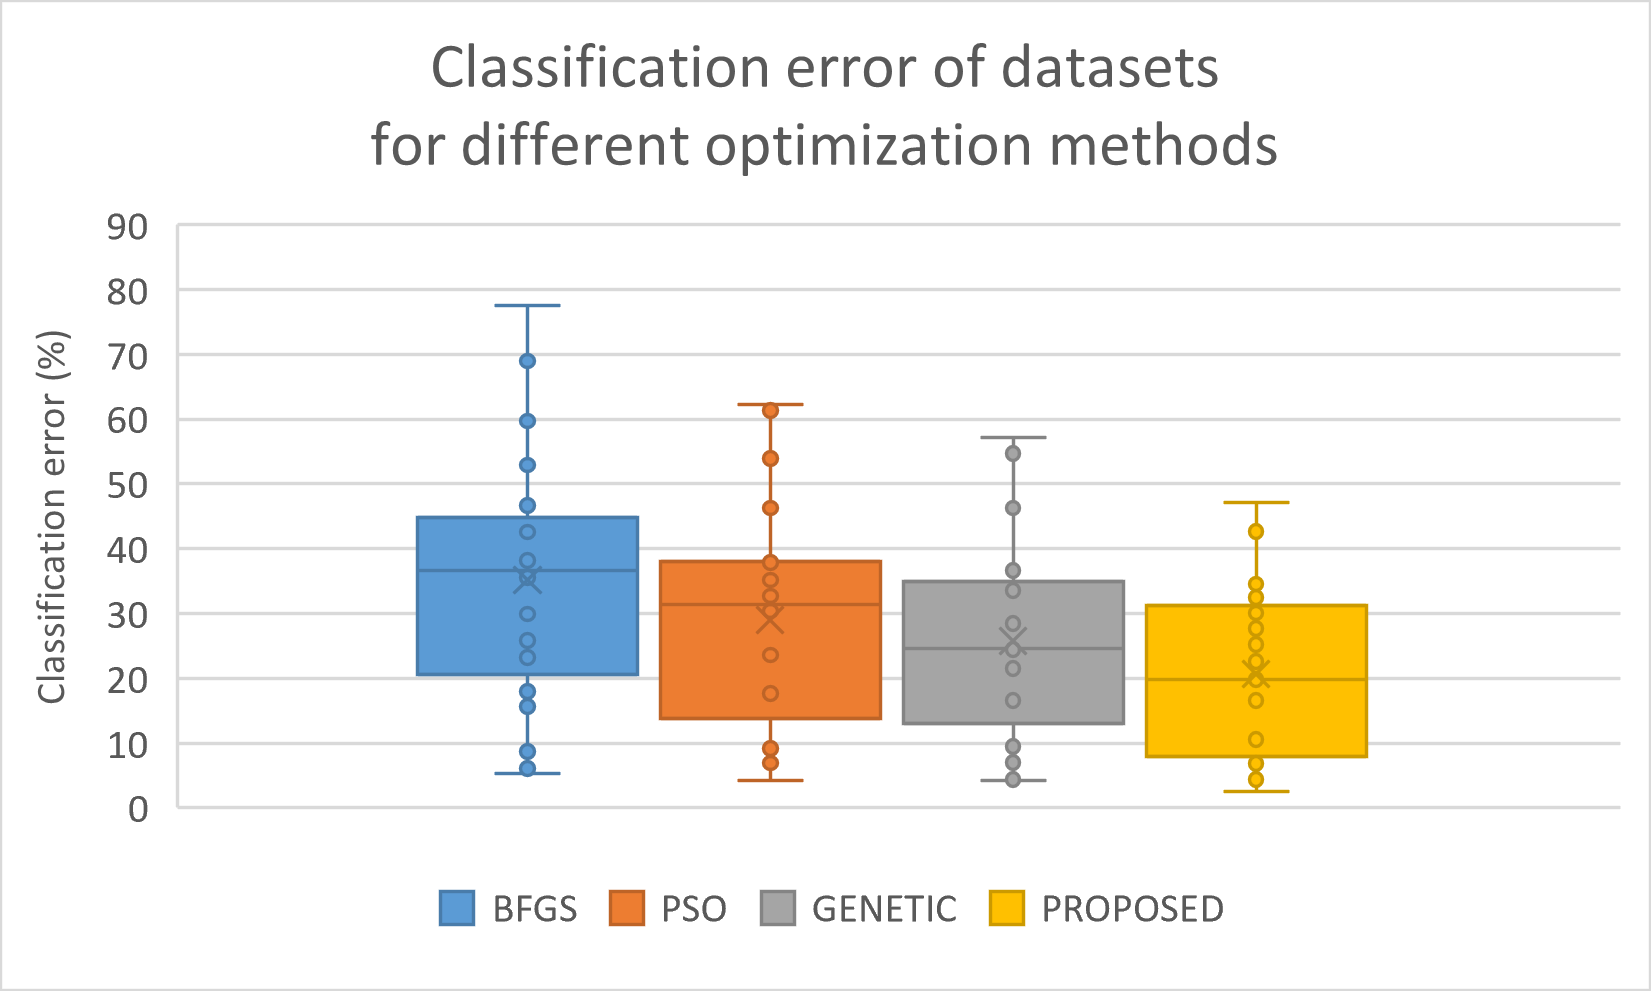
\includegraphics{stat_class}

\caption{Statistical comparison of the used optimization methods for the classification
datasets.\label{fig:statClass}}
\end{figure}

\begin{figure}[H]
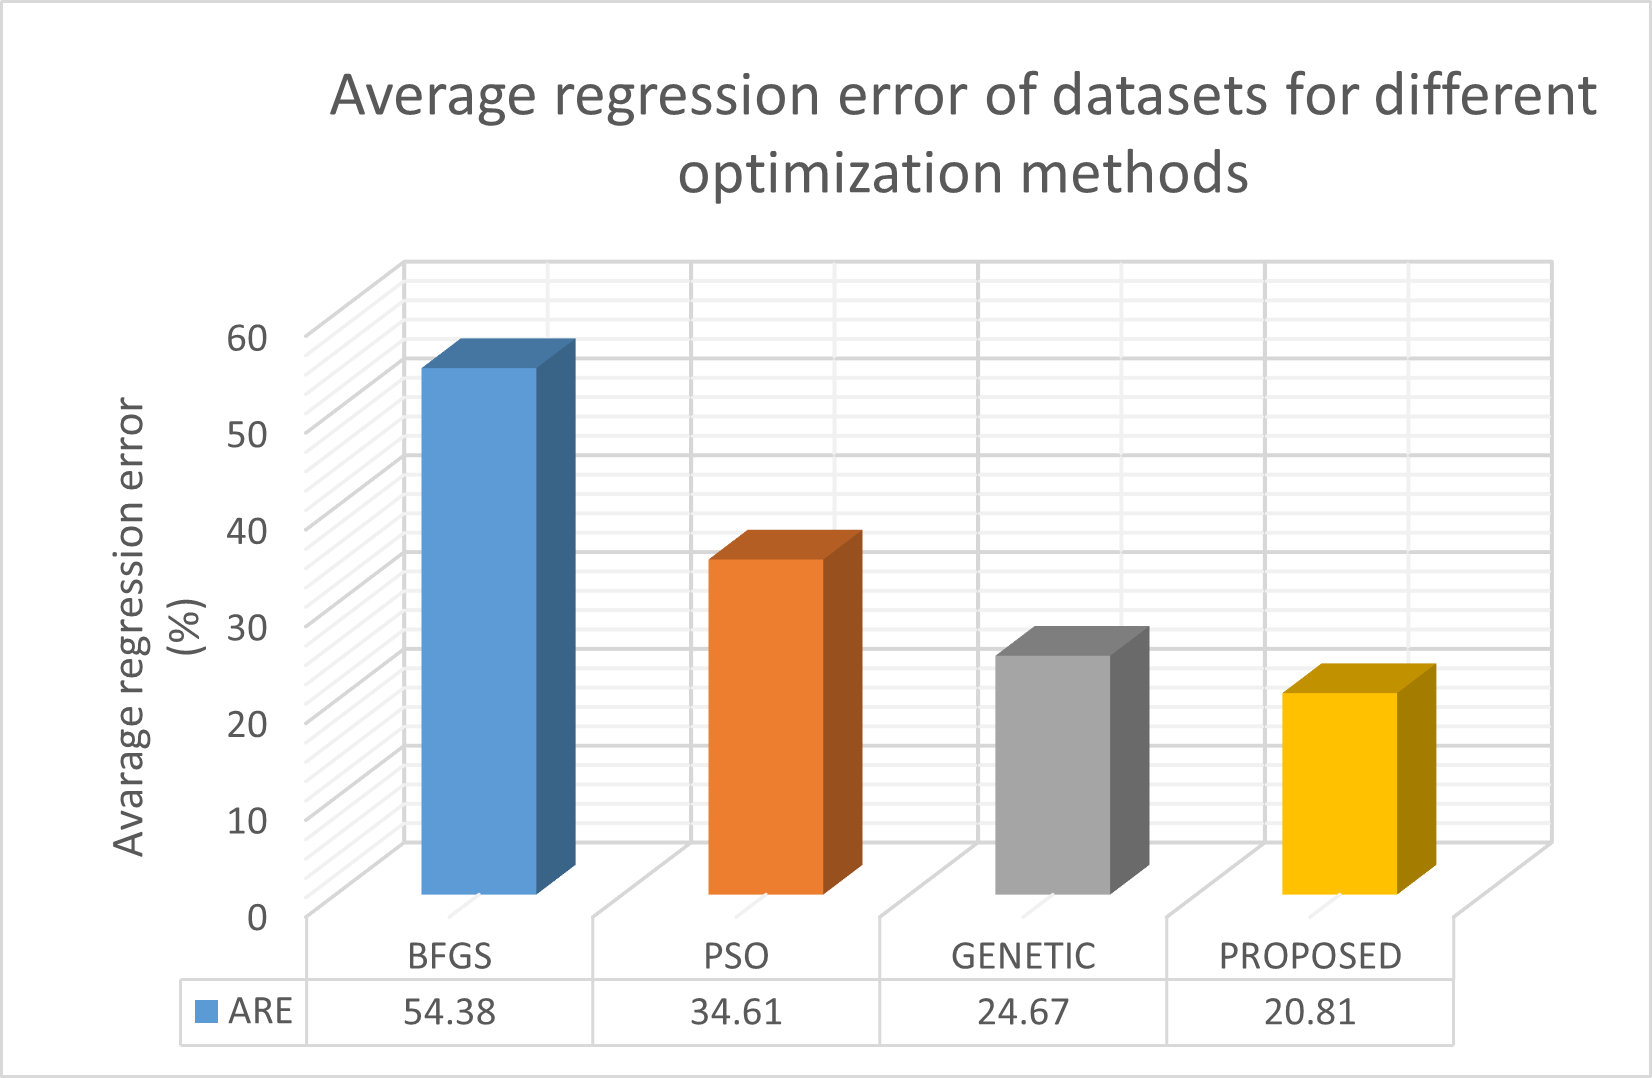
\includegraphics{stat_regression}

\caption{Statistical comparison of the used methods for the regression datasets.\label{fig:statRegression}}

\end{figure}
As the comparison of the experimental results and their statistical
comparison shows, the genetic algorithm method significantly outperforms
the others in terms of accuracy. However, the proposed technique,
which is an extension of genetic algorithms, significantly improves
their performance on almost all datasets. In several datasets, the
reduction in error in the test set can reach up to 80\% compared to
genetic algorithms.

Additionally, in order to explore the stability and the robustness
of the proposed method, further experiments were conducted with different
values for the critical parameters of the method. The results in Table
\ref{tab:experF} depict the application of the proposed method on
classification datasets, with different values for the critical parameter
$F$, which controls the magnitude of changes in the Simulated Annealing
variant. Also, the statistical comparison for the average classification
error is shown in Figure \ref{fig:statF}.

\begin{table}[H]
\caption{Experimental results using different values for the critical parameter
$F$. The experiments were executed on the classification datasets.\label{tab:experF}}

\begin{centering}
\begin{tabular}{|c|c|c|c|}
\hline 
DATASET & $F=0.05$ & $F=0.10$ & $F=0.15$\tabularnewline
\hline 
\hline 
APPENDICITIS & 22.30\% & 22.60\% & 24.20\%\tabularnewline
\hline 
AUSTRALIAN & 33.78\% & 32.42\% & 28.72\%\tabularnewline
\hline 
BALANCE & 8.16\% & 8.10\% & 8.26\%\tabularnewline
\hline 
BANDS & 34.81\% & 34.53\% & 33.97\%\tabularnewline
\hline 
CIRCULAR & 4.22\% & 4.35\% & 4.38\%\tabularnewline
\hline 
CLEVELAND & 46.24\% & 42.62\% & 44.58\%\tabularnewline
\hline 
DERMATOLOGY & 16.69\% & 12.12\% & 9.94\%\tabularnewline
\hline 
ECOLI & 50.64\% & 47.18\% & 45.24\%\tabularnewline
\hline 
FERT & 26.60\% & 25.20\% & 25.90\%\tabularnewline
\hline 
HEART & 23.96\% & 16.59\% & 15.15\%\tabularnewline
\hline 
HEARTATTACK & 25.70\% & 20.13\% & 19.97\%\tabularnewline
\hline 
HOUSEVOTES & 6.74\% & 7.13\% & 7.44\%\tabularnewline
\hline 
LIVERDISORDER & 34.50\% & 32.88\% & 32.50\%\tabularnewline
\hline 
PARKINSONS & 16.53\% & 16.63\% & 15.68\%\tabularnewline
\hline 
PIMA & 33.18\% & 30.08\% & 26.33\%\tabularnewline
\hline 
POPFAILURES & 4.52\% & 5.44\% & 5.89\%\tabularnewline
\hline 
REGIONS2 & 30.86\% & 27.69\% & 26.40\%\tabularnewline
\hline 
SAHEART & 35.68\% & 34.56\% & 32.67\%\tabularnewline
\hline 
SEGMENT & 32.53\% & 28.41\% & 26.15\%\tabularnewline
\hline 
SONAR & 21.40\% & 19.80\% & 19.80\%\tabularnewline
\hline 
SPIRAL & 45.15\% & 44.54\% & 44.23\%\tabularnewline
\hline 
WDBC & 7.38\% & 5.66\% & 4.91\%\tabularnewline
\hline 
WINE & 16.06\% & 10.59\% & 8.82\%\tabularnewline
\hline 
Z\_F\_S & 18.20\% & 11.10\% & 8.60\%\tabularnewline
\hline 
ZO\_NF\_S & 16.80\% & 6.86\% & 6.22\%\tabularnewline
\hline 
ZONF\_S & 2.92\% & 2.48\% & 2.42\%\tabularnewline
\hline 
ZOO & 7.60\% & 7.60\% & 6.80\%\tabularnewline
\hline 
\textbf{AVERAGE} & \textbf{23.08\%} & \textbf{20.64\%} & \textbf{19.82\%}\tabularnewline
\hline 
\end{tabular}
\par\end{centering}
\end{table}

\begin{figure}[H]
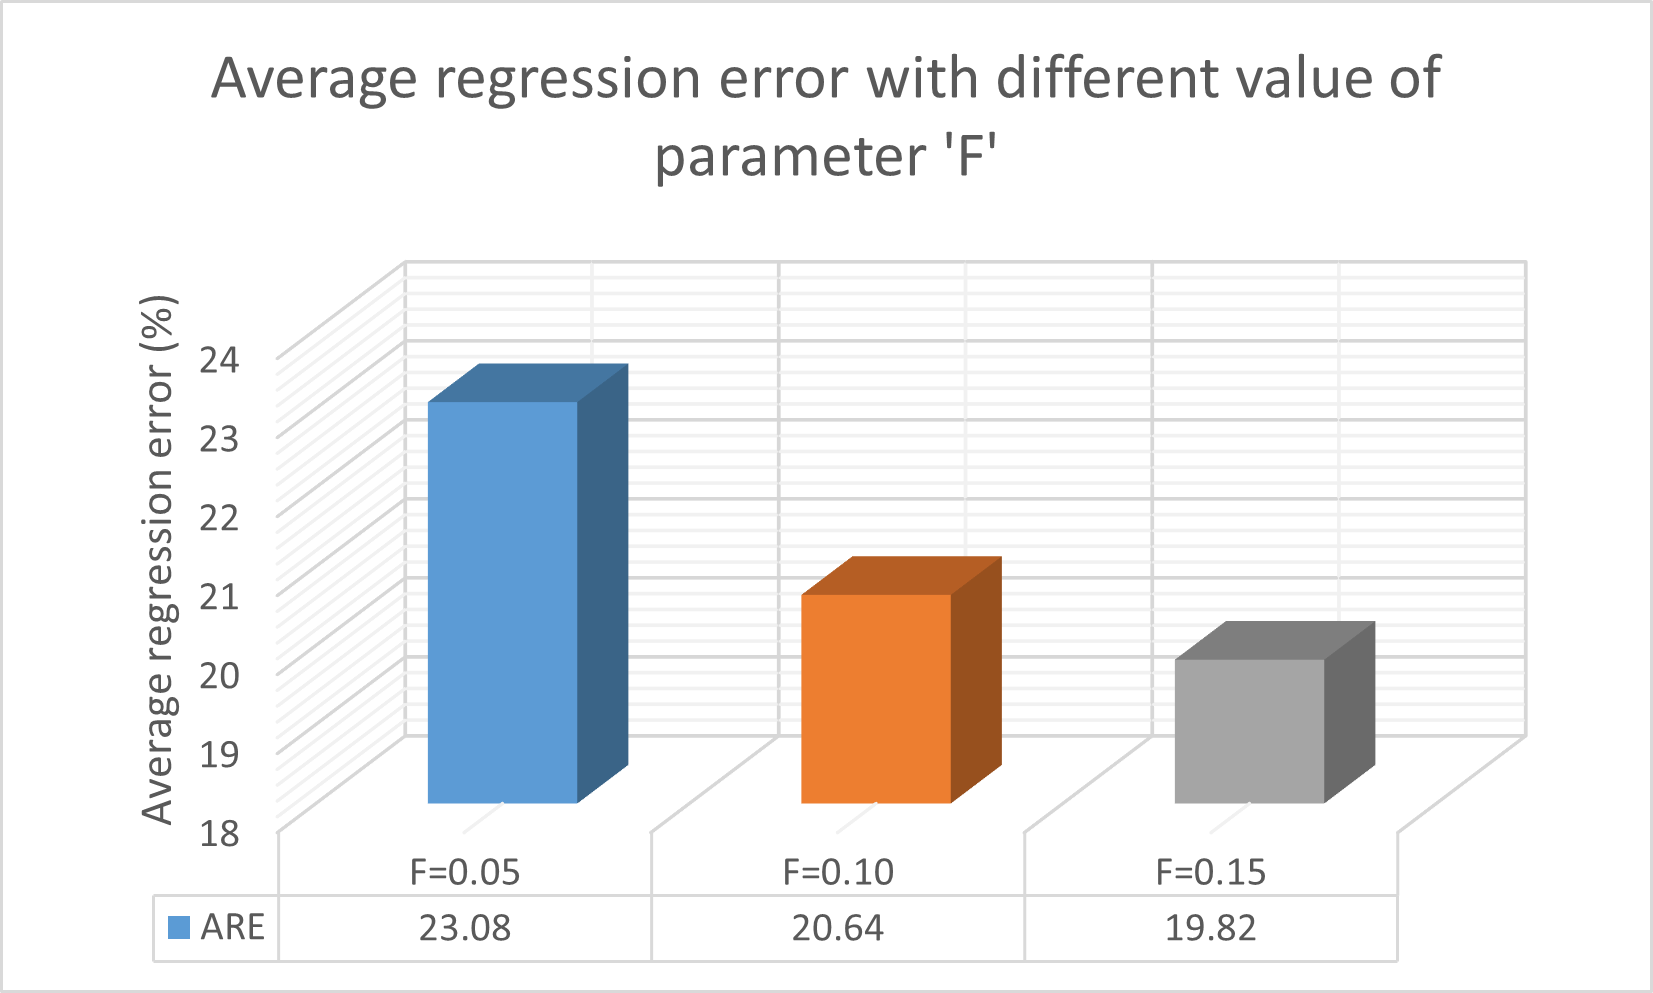
\includegraphics{stat_paramF}

\caption{Statistical comparison for the results obtained by the proposed method
for different values of the critical parameter $F$\label{fig:statF}}

\end{figure}
The proposed method is shown to improve when the critical parameter
$F$ increases from 0.05 to 0.10 but does not improve further for
a larger increase in the value of the parameter. Therefore, for small
changes in chromosome values there is no significant improvement from
applying the minimization technique, but larger variations yield more
significant reductions in classification error. Also, an experiment
was conducted using different values for the parameter $N_{R}$, which
determines the number of changes in the chromosomes. The results for
this experiment and for the classification datasets are shown in Table
\ref{tab:experNR} and the statistical comparison is shown in Figure
\ref{fig:statNR}.

\begin{table}[H]
\caption{Experiments using the parameter $N_{R}$ of the proposed algorithm.
The experiments were performed by applying the proposed method on
the used classification datasets.\label{tab:experNR}}

\begin{centering}
\begin{tabular}{|c|c|c|c|}
\hline 
DATASET & $N_{R}=10$ & $N_{R}=20$ & $N_{R}=30$\tabularnewline
\hline 
\hline 
APPENDICITIS & 23.70\% & 22.60\% & 22.50\%\tabularnewline
\hline 
AUSTRALIAN & 32.60\% & 32.42\% & 31.51\%\tabularnewline
\hline 
BALANCE & 8.36\% & 8.10\% & 8.05\%\tabularnewline
\hline 
BANDS & 34.28\% & 34.53\% & 33.75\%\tabularnewline
\hline 
CIRCULAR & 4.48\% & 4.35\% & 4.51\%\tabularnewline
\hline 
CLEVELAND & 43.38\% & 42.62\% & 43.24\%\tabularnewline
\hline 
DERMATOLOGY & 13.97\% & 12.12\% & 11.26\%\tabularnewline
\hline 
ECOLI & 47.79\% & 47.18\% & 47.06\%\tabularnewline
\hline 
FERT & 26.50\% & 25.20\% & 26.70\%\tabularnewline
\hline 
HEART & 20.67\% & 16.59\% & 16.18\%\tabularnewline
\hline 
HEARTATTACK & 23.20\% & 20.13\% & 20.43\%\tabularnewline
\hline 
HOUSEVOTES & 7.30\% & 7.13\% & 7.44\%\tabularnewline
\hline 
LIVERDISORDER & 32.50\% & 32.88\% & 33.09\%\tabularnewline
\hline 
PARKINSONS & 16.63\% & 16.63\% & 15.26\%\tabularnewline
\hline 
PIMA & 31.89\% & 30.08\% & 28.04\%\tabularnewline
\hline 
POPFAILURES & 4.43\% & 5.44\% & 5.48\%\tabularnewline
\hline 
REGIONS2 & 29.71\% & 27.69\% & 26.99\%\tabularnewline
\hline 
SAHEART & 34.28\% & 34.56\% & 33.26\%\tabularnewline
\hline 
SEGMENT & 29.19\% & 28.41\% & 27.46\%\tabularnewline
\hline 
SONAR & 20.95\% & 19.80\% & 20.05\%\tabularnewline
\hline 
SPIRAL & 44.17\% & 44.54\% & 44.20\%\tabularnewline
\hline 
WDBC & 6.48\% & 5.66\% & 5.45\%\tabularnewline
\hline 
WINE & 12.76\% & 10.59\% & 10.41\%\tabularnewline
\hline 
Z\_F\_S & 13.50\% & 11.10\% & 8.70\%\tabularnewline
\hline 
ZO\_NF\_S & 15.14\% & 6.86\% & 7.28\%\tabularnewline
\hline 
ZONF\_S & 2.44\% & 2.48\% & 2.38\%\tabularnewline
\hline 
ZOO & 7.40\% & 7.60\% & 7.60\%\tabularnewline
\hline 
\textbf{AVERAGE} & \textbf{21.77\%} & \textbf{20.64\%} & \textbf{20.31\%}\tabularnewline
\hline 
\end{tabular}
\par\end{centering}
\end{table}

\begin{figure}[H]
\begin{centering}
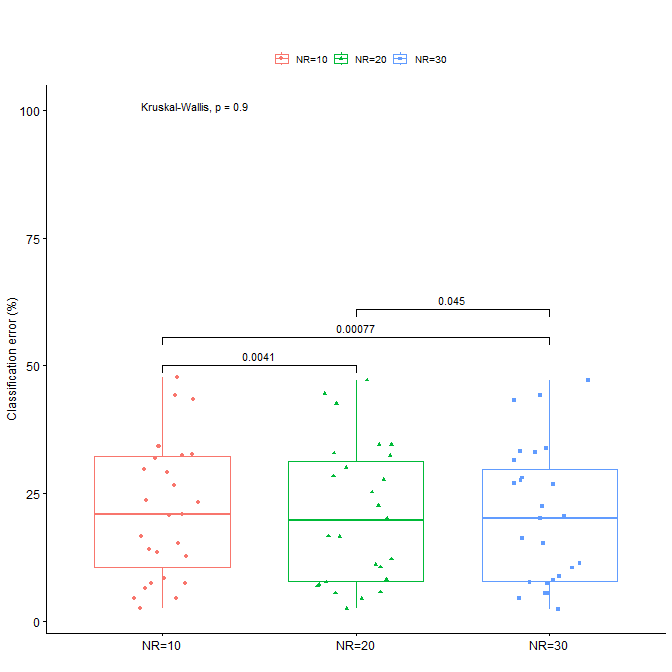
\includegraphics[scale=0.5]{stat_NR}
\par\end{centering}
\caption{Statistical comparison for the results obtained by the proposed method
as applied on the classification datasets, using different values
of the parameter $N_{R}$.\label{fig:statNR}}

\end{figure}
In the case of this parameter, no noticeable differences are observed
as the value of the parameter increases. This means that even a limited
number of changes (e.g. 10-20) can yield significant reductions in
classification errors. Finally, an experiment was conducted to measure
the effect of the parameter $N_{I}$ to the produced results. The
experimental results for different values of the $N_{I}$ parameter
are shown in Table \ref{tab:experNI} and the statistical comparison
is depicted in Figure \ref{fig:statNI}.

\begin{table}[H]
\caption{Experiments using the proposed method on the classification datasets
for various values of the parameter $N_{I}$.\label{tab:experNI}}

\centering{}%
\begin{tabular}{|c|c|c|c|}
\hline 
DATASET & $L_{I}=10$ & $L_{I}=20$ & $L_{I}=30$\tabularnewline
\hline 
\hline 
APPENDICITIS & 24.20\% & 22.60\% & 24.10\%\tabularnewline
\hline 
AUSTRALIAN & 30.49\% & 32.42\% & 33.22\%\tabularnewline
\hline 
BALANCE & 8.50\% & 8.10\% & 8.44\%\tabularnewline
\hline 
BANDS & 34.08\% & 34.53\% & 34.22\%\tabularnewline
\hline 
CIRCULAR & 4.29\% & 4.35\% & 4.36\%\tabularnewline
\hline 
CLEVELAND & 44.58\% & 42.62\% & 43.10\%\tabularnewline
\hline 
DERMATOLOGY & 10.63\% & 12.12\% & 12.54\%\tabularnewline
\hline 
ECOLI & 45.24\% & 47.18\% & 47.67\%\tabularnewline
\hline 
FERT & 25.90\% & 25.20\% & 27.30\%\tabularnewline
\hline 
HEART & 15.44\% & 16.59\% & 19.26\%\tabularnewline
\hline 
HEARTATTACK & 19.87\% & 20.13\% & 21.83\%\tabularnewline
\hline 
HOUSEVOTES & 7.44\% & 7.13\% & 6.65\%\tabularnewline
\hline 
LIVERDISORDER & 32.50\% & 32.88\% & 32.85\%\tabularnewline
\hline 
PARKINSONS & 15.89\% & 16.63\% & 15.79\%\tabularnewline
\hline 
PIMA & 28.96\% & 30.08\% & 31.28\%\tabularnewline
\hline 
POPFAILURES & 5.13\% & 5.44\% & 4.76\%\tabularnewline
\hline 
REGIONS2 & 25.74\% & 27.69\% & 28.98\%\tabularnewline
\hline 
SAHEART & 32.67\% & 34.56\% & 34.33\%\tabularnewline
\hline 
SEGMENT & 26.55\% & 28.41\% & 28.62\%\tabularnewline
\hline 
SONAR & 19.80\% & 19.80\% & 21.69\%\tabularnewline
\hline 
SPIRAL & 43.82\% & 44.54\% & 43.85\%\tabularnewline
\hline 
WDBC & 5.48\% & 5.66\% & 5.95\%\tabularnewline
\hline 
WINE & 8.82\% & 10.59\% & 11.65\%\tabularnewline
\hline 
Z\_F\_S & 8.60\% & 11.10\% & 12.13\%\tabularnewline
\hline 
ZO\_NF\_S & 6.22\% & 6.86\% & 9.06\%\tabularnewline
\hline 
ZONF\_S & 2.42\% & 2.48\% & 2.64\%\tabularnewline
\hline 
ZOO & 6.80\% & 7.60\% & 7.10\%\tabularnewline
\hline 
\textbf{AVERAGE} & \textbf{20.00\%} & \textbf{20.64\%} & \textbf{21.24\%}\tabularnewline
\hline 
\end{tabular}
\end{table}

\begin{figure}[H]
\begin{centering}
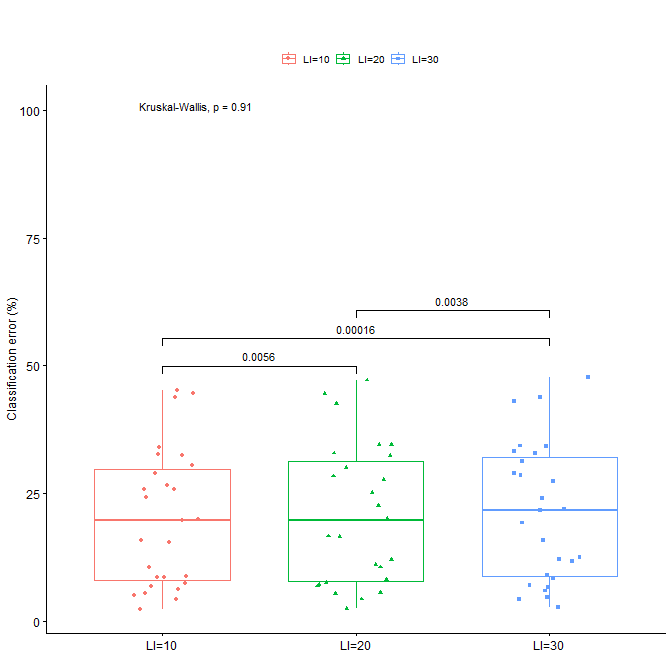
\includegraphics[scale=0.5]{stat_LI}
\par\end{centering}
\caption{Statistical comparison for the results obtained by the proposed method
as applied on the classification datasets, using different values
of the parameter $L_{I}$.\label{fig:statNI}}

\end{figure}
Once again, the performance of the proposed technique appears not
to be significantly affected by the change of parameter $N_{I}$.
The method performs slightly better for lower values of the $N_{I}$
parameter, since the smaller this parameter is, the more often the
variant of Simulated Annealing will be applied to the genetic population.
However, this reduction is limited and therefore there does not appear
to be a drastic effect of this particular parameter on the behavior
of the algorithm.

\section{Conclusions\label{sec:Conclusions}}

A new variant of the Simulated Annealing method is introduced in the
current work, which aims to improve the effectiveness of Genetic Algorithms
in the task of training neural networks. This new method improves
the performance of genetic population chromosomes, which are randomly
selected from the population. This method brings random changes to
the selected chromosomes and the course of the optimization is determined
by parameters, such as the temperature of the method. For high temperature
values, the method accepts error values that may be higher than the
initial one, in order to achieve the optimal exploration of the research
space, but as the temperature decreases, the method focuses on the
optimal values of the error function. The new training method is quite
general and has been successfully applied to a variety of data classification
and data fitting problems. This new technique significantly improves
the performance of Genetic Algorithms in almost all data sets that
were used, and in fact, in several of them the reduction in the error
can reach up to 80\%. Furthermore, the technique's behavior and performance
are not significantly affected by any variations in its critical parameters
except for the $F$ parameter, which controls the magnitude of changes
that can be made to a chromosome. However, the effect of this parameter
seems to decrease for large values. 

However, this new technique may affect the execution time of the Genetic
Algorithm as it adds a new computational part. This overhead in computational
time may be reduced by using modern parallel programming techniques
from recent literature \citep{psa}. Furthermore, the effect of the
temperature reduction mechanism on the performance of the Simulated
Annealing variant could be studied and more sophisticated minimization
techniques could be tested. Also, an effort could be made to apply
the new technical training to other machine learning models, as, for
example, the Radial Basis Function (RBF) networks \citep{rbf1}.

\vspace{6pt}


\authorcontributions{V.C. and I.G.T. conducted the experiments, employing several datasets
and provided the comparative experiments. D.T. and V.C. performed
the statistical analysis and prepared the manuscript. All authors
have read and agreed to the published version of the manuscript.}

\funding{This research received no external funding.}

\institutionalreview{Not applicable.}

\informedconsent{Not applicable.}

\dataavailability{Not applicable. }

\acknowledgments{This research has been financed by the European Union : Next Generation
EU through the Program Greece 2.0 National Recovery and Resilience
Plan , under the call RESEARCH -- CREATE -- INNOVATE, project name
“iCREW: Intelligent small craft simulator for advanced crew training
using Virtual Reality techniques\textquotedbl{} (project code:TAEDK-06195).}

\conflictsofinterest{The authors declare no conflicts of interest.}

\appendixtitles{no}

\begin{adjustwidth}{-\extralength}{0cm}{}


\reftitle{References}
\begin{thebibliography}{999}
\bibitem{nn1}C. Bishop, Neural Networks for Pattern Recognition,
Oxford University Press, 1995.

\bibitem{nn2}G. Cybenko, Approximation by superpositions of a sigmoidal
function, Mathematics of Control Signals and Systems \textbf{2}, pp.
303-314, 1989.

\bibitem{nnphysics1}P. Baldi, K. Cranmer, T. Faucett et al, Parameterized
neural networks for high-energy physics, Eur. Phys. J. C \textbf{76},
2016.

\bibitem{nnphysics2}J. J. Valdas and G. Bonham-Carter, Time dependent
neural network models for detecting changes of state in complex processes:
Applications in earth sciences and astronomy, Neural Networks \textbf{19},
pp. 196-207, 2006

\bibitem{nnphysics3}G. Carleo,M. Troyer, Solving the quantum many-body
problem with artificial neural networks, Science \textbf{355}, pp.
602-606, 2017.

\bibitem{nnchem1}Lin Shen, Jingheng Wu, and Weitao Yang, Multiscale
Quantum Mechanics/Molecular Mechanics Simulations with Neural Networks,
Journal of Chemical Theory and Computation \textbf{12}, pp. 4934-4946,
2016.

\bibitem{nnchem2}Sergei Manzhos, Richard Dawes, Tucker Carrington,
Neural network‐based approaches for building high dimensional and
quantum dynamics‐friendly potential energy surfaces, Int. J. Quantum
Chem. \textbf{115}, pp. 1012-1020, 2015.

\bibitem{nnchem3}Jennifer N. Wei, David Duvenaud, and Alán Aspuru-Guzik,
Neural Networks for the Prediction of Organic Chemistry Reactions,
ACS Central Science \textbf{2}, pp. 725-732, 2016.

\bibitem{nnecon1}Lukas Falat and Lucia Pancikova, Quantitative Modelling
in Economics with Advanced Artificial Neural Networks, Procedia Economics
and Finance \textbf{34}, pp. 194-201, 2015.

\bibitem{nnecon2}Mohammad Namazi, Ahmad Shokrolahi, Mohammad Sadeghzadeh
Maharluie, Detecting and ranking cash flow risk factors via artificial
neural networks technique, Journal of Business Research \textbf{69},
pp. 1801-1806, 2016.

\bibitem{nncecon3}G. Tkacz, Neural network forecasting of Canadian
GDP growth, International Journal of Forecasting \textbf{17}, pp.
57-69, 2001.

\bibitem{nnmed1}Igor I. Baskin, David Winkler and Igor V. Tetko,
A renaissance of neural networks in drug discovery, Expert Opinion
on Drug Discovery \textbf{11}, pp. 785-795, 2016.

\bibitem{nnmed2}Ronadl Bartzatt, Prediction of Novel Anti-Ebola Virus
Compounds Utilizing Artificial Neural Network (ANN), Chemistry Faculty
Publications \textbf{49}, pp. 16-34, 2018.

\bibitem{nn_flood}M.B. Kia, S. Pirasteh, B. Pradhan B. et al, An
artificial neural network model for flood simulation using GIS: Johor
River Basin, Malaysia, Environ Earth Sci \textbf{67}, pp. 251--264,
2012.

\bibitem{nn_solar}A.K. Yadav, S.S. Chandel, Solar radiation prediction
using Artificial Neural Network techniques: A review, Renewable and
Sustainable Energy Reviews \textbf{33}, pp. 772-781, 2014.

\bibitem{nn_agro}M.A. Getahun, S.M. Shitote, C. Zachary, Artificial
neural network based modelling approach for strength prediction of
concrete incorporating agricultural and construction wastes, Construction
and Building Materials \textbf{190}, pp. 517-525, 2018.

\bibitem{nn_wireless}M. Chen, U. Challita, W. Saad, C. Yin and M.
Debbah, Artificial Neural Networks-Based Machine Learning for Wireless
Networks: A Tutorial, IEEE Communications Surveys \& Tutorials \textbf{21},
pp. 3039-3071, 2019.

\bibitem{nnc}I.G. Tsoulos, D. Gavrilis, E. Glavas, Neural network
construction and training using grammatical evolution, Neurocomputing
\textbf{72}, pp. 269-277, 2008.

\bibitem{bpnn}D.E. Rumelhart, G.E. Hinton and R.J. Williams, Learning
representations by back-propagating errors, Nature \textbf{323}, pp.
533 - 536 , 1986.

\bibitem{bpnn2}T. Chen and S. Zhong, Privacy-Preserving Backpropagation
Neural Network Learning, IEEE Transactions on Neural Networks \textbf{20},
, pp. 1554-1564, 2009.

\bibitem{nn_leve}B. M. Wilamowski, S. Iplikci, O. Kaynak and M. O.
Efe, \textquotedbl An algorithm for fast convergence in training
neural networks,\textquotedbl{} IJCNN'01. International Joint Conference
on Neural Networks. Proceedings (Cat. No.01CH37222), Washington, DC,
USA, 2001, pp. 1778-1782 vol.3, doi: 10.1109/IJCNN.2001.938431.

\bibitem{rpropnn}M. Riedmiller and H. Braun, A Direct Adaptive Method
for Faster Backpropagation Learning: The RPROP algorithm, Proc. of
the IEEE Intl. Conf. on Neural Networks, San Francisco, CA, pp. 586--591,
1993.

\bibitem{rpropnn3}T. Pajchrowski, K. Zawirski and K. Nowopolski,
Neural Speed Controller Trained Online by Means of Modified RPROP
Algorithm, IEEE Transactions on Industrial Informatics \textbf{11},
pp. 560-568, 2015.

\bibitem{rpropnn2}Rinda Parama Satya Hermanto, Suharjito, Diana,
Ariadi Nugroho, Waiting-Time Estimation in Bank Customer Queues using
RPROP Neural Networks, Procedia Computer Science \textbf{ 135}, pp.
35-42, 2018.

\bibitem{quasinn}B. Robitaille and B. Marcos and M. Veillette and
G. Payre, Modified quasi-Newton methods for training neural networks,
Computers \& Chemical Engineering \textbf{20}, pp. 1133-1140, 1996.

\bibitem{quasinn2}Q. Liu, J. Liu, R. Sang, J. Li, T. Zhang and Q.
Zhang, Fast Neural Network Training on FPGA Using Quasi-Newton Optimization
Method,IEEE Transactions on Very Large Scale Integration (VLSI) Systems
\textbf{26}, pp. 1575-1579, 2018.

\bibitem{psonn}C. Zhang, H. Shao and Y. Li, Particle swarm optimisation
for evolving artificial neural network, IEEE International Conference
on Systems, Man, and Cybernetics, , pp. 2487-2490, 2000.

\bibitem{psonn2}Jianbo Yu, Shijin Wang, Lifeng Xi, Evolving artificial
neural networks using an improved PSO and DPSO \textbf{71}, pp. 1054-1060,
2008.

\bibitem{nn_de}J. Ilonen, J.K. Kamarainen, J. Lampinen, Differential
Evolution Training Algorithm for Feed-Forward Neural Networks. Neural
Processing Letters \textbf{17}, pp. 93--105, 2003.

\bibitem{nn_survey}Le Zhang and P.N. Suganthan, A survey of randomized
algorithms for training neural networks, Information Sciences \textbf{364-365},
pp. 146-155, 2016.

\bibitem{nnhybrid1}M. Yaghini, M.M. Khoshraftar, M. Fallahi, A hybrid
algorithm for artificial neural network training, Engineering Applications
of Artificial Intelligence \textbf{26}, pp 293-301, 2013.

\bibitem{nnhybrid2}J.F. Chen, Q.H. Do,H.N. Hsieh, Training Artificial
Neural Networks by a Hybrid PSO-CS Algorithm, Algorithms \textbf{8},
pp. 292-308, 2015.

\bibitem{csmethod}X.S. Yang, S. Deb, Engineering Optimisation by
Cuckoo Search, Int. J. Math. Model. Numer. Optim. \textbf{1}, 330--343,
2010.

\bibitem{nninit1}I. Ivanova, M. Kubat, Initialization of neural networks
by means of decision trees, Knowledge-Based Systems \textbf{8}, pp.
333-344, 1995.

\bibitem{weight_init2}J.Y.F. Yam, T.W.S. Chow, A weight initialization
method for improving training speed in feedforward neural network,
Neurocomputing \textbf{30}, pp. 219-232, 2000.

\bibitem{weight_init3}K. Chumachenko, A. Iosifidis, M. Gabbouj, Feedforward
neural networks initialization based on discriminant learning, Neural
Networks \textbf{146}, pp. 220-229, 2022.

\bibitem{nninitreview}M.V. Narkhede, P.P. Bartakke, M.S. Sutaone,
A review on weight initialization strategies for neural networks,
Artif Intell Rev \textbf{55}, pp. 291--322, 2022.

\bibitem{nn_gpu1}K-S Oh, K. Jung, GPU implementation of neural networks,
Pattern Recognition \textbf{37}, pp. 1311-1314, 2004.

\bibitem{nn_gpu2}A.A. Huqqani, E.Schikuta, S. Ye, P. Chen, Multicore
and GPU Parallelization of Neural Networks for Face Recognition, Procedia
Computer Science \textbf{18}, pp. 349-358, 2013.

\bibitem{nn_gpu3}M. Zhang, K. Hibi, J. Inoue, GPU-accelerated artificial
neural network potential for molecular dynamics simulation, Computer
Physics Communications \textbf{285}, 108655, 2023.

\bibitem{nn_gpu_review}Pallipuram, V.K., Bhuiyan, M. \& Smith, M.C.
A comparative study of GPU programming models and architectures using
neural networks. J Supercomput \textbf{61}, 673--718, 2012.

\bibitem{Holland} Holland, J.H. Genetic algorithms. Sci. Am. \textbf{267},
66--73, 1992.

\bibitem{Stender} Stender, J. Parallel Genetic Algorithms: Theory
\& Applications; IOS Press: Amsterdam, The Netherlands, 1993.

\bibitem{Goldberg} Goldberg, D. Genetic Algorithms in Search, Optimization
and Machine Learning; Addison-Wesley Publishing Company: Reading,
MA, USA, 1989.

\bibitem{Michaelewicz} Michaelewicz, Z. Genetic Algorithms + Data
Structures = Evolution Programs; Springer: Berlin/Heidelberg, Germany,
1996.

\bibitem{ga_problem1}Y.H. Santana, R.M. Alonso, G.G. Nieto, L. Martens,
W. Joseph, D. Plets, Indoor genetic algorithm-based 5G network planning
using a machine learning model for path loss estimation, Appl. Sci.
\textbf{12}, 3923. 2022.

\bibitem{ga_problem2}X. Liu, D. Jiang, B. Tao, G. Jiang, Y. Sun,
J. Kong, B. Chen, Genetic algorithm-based trajectory optimization
for digital twin robots, Front. Bioeng. Biotechnol \textbf{9}, 793782,
2022.

\bibitem{ga_problem3}K. Nonoyama, Z.Liu, T. Fujiwara, M.M. Alam,
T. Nishi, Energy-efficient robot configuration and motion planning
using genetic algorithm and particle swarm optimization, Energies
\textbf{15}, 2074, 2022.

\bibitem{ga_problem4}K. Liu, B. Deng, Q. Shen, J. Yang, Y. Li, Optimization
based on genetic algorithms on energy conservation potential of a
high speed SI engine fueled with butanol--gasoline blends, Energy
Rep. \textbf{8}, pp. 69--80, 2022.

\bibitem{ga_problem5}G. Zhou, S. Zhu, S. Luo, Location optimization
of electric vehicle charging stations: Based on cost model and genetic
algorithm, Energy \textbf{247}, 123437, 2022.

\bibitem{siman_main}S. Kirkpatrick, C.D. Gelatt Jr, M.P. Vecchi,
Optimization by simulated annealing, Science \textbf{220}, pp. 671-680,
1983.

\bibitem{siman_problem1}S.J. D'Amico, S-J. Wang, R. Batta, C.M. Rump,
A simulated annealing approach to police district design Computers
\& Operations Research \textbf{29}, pp. 667-684, 2002.

\bibitem{siman_problem2}Y. Crama, M. Schyns, Simulated annealing
for complex portfolio selection problems\}, journal = \{European Journal
of Operational Research \textbf{150}, pp. 546-571, 2003.

\bibitem{siman_problem3}K.M. El-Naggar, M.R. AlRashidi, M.F. AlHajri,
A.K. Al-Othman, Simulated Annealing algorithm for photovoltaic parameters
identification, Solar Energy \textbf{86}, pp. 266-274, 2012.

\bibitem{ga_drug}L. Terfloth, J. Gasteiger, Neural networks and genetic
algorithms in drug design, Drug Discovery Today \textbf{6}, pp. 102-108,
2001.

\bibitem{ga_gear}B. Samanta, Artificial neural networks and genetic
algorithms for gear fault detection, Mechanical Systems and Signal
Processing \textbf{18}, pp. 1273-1282, 2004.

\bibitem{ga_forecasting}F. Yu, X. Xu, A short-term load forecasting
model of natural gas based on optimized genetic algorithm and improved
BP neural network, Applied Energy \textbf{134}, pp. 102-113, 2014.

\bibitem{kaelo}P. Kaelo, M.M. Ali, Integrated crossover rules in
real coded genetic algorithms, European Journal of Operational Research
\textbf{176}, pp. 60-76, 2007.

\bibitem{Powell}M.J.D Powell, A Tolerant Algorithm for Linearly Constrained
Optimization Calculations, Mathematical Programming \textbf{45}, pp.
547-566, 1989. 

\bibitem{UCL}M. Kelly, R. Longjohn, K. Nottingham, The UCI Machine
Learning Repository. 2023. Available online: https://archive.ics.uci.edu
(accessed on 18 February 2024).

\bibitem{Keel}J. Alcalá-Fdez, A. Fernandez, J. Luengo, J. Derrac,
S. García, L. Sánchez, F. Herrera. KEEL Data-Mining Software Tool:
Data Set Repository, Integration of Algorithms and Experimental Analysis
Framework. Journal of Multiple-Valued Logic and Soft Computing 17,
pp. 255-287, 2011.

\bibitem{appendicitis}Weiss, Sholom M. and Kulikowski, Casimir A.,
Computer Systems That Learn: Classification and Prediction Methods
from Statistics, Neural Nets, Machine Learning, and Expert Systems,
Morgan Kaufmann Publishers Inc, 1991.

\bibitem{australian}J.R. Quinlan, Simplifying Decision Trees. International
Journal of Man-Machine Studies \textbf{27}, pp. 221-234, 1987. 

\bibitem{balance}T. Shultz, D. Mareschal, W. Schmidt, Modeling Cognitive
Development on Balance Scale Phenomena, Machine Learning \textbf{16},
pp. 59-88, 1994.

\bibitem{cleveland1}Z.H. Zhou,Y. Jiang, NeC4.5: neural ensemble based
C4.5,\textquotedbl{} in IEEE Transactions on Knowledge and Data Engineering
\textbf{16}, pp. 770-773, 2004.

\bibitem{cleveland2}R. Setiono , W.K. Leow, FERNN: An Algorithm for
Fast Extraction of Rules from Neural Networks, Applied Intelligence
\textbf{12}, pp. 15-25, 2000.

\bibitem{dermatology}G. Demiroz, H.A. Govenir, N. Ilter, Learning
Differential Diagnosis of Eryhemato-Squamous Diseases using Voting
Feature Intervals, Artificial Intelligence in Medicine. \textbf{13},
pp. 147--165, 1998.

\bibitem{ecoli}P. Horton, K.Nakai, A Probabilistic Classification
System for Predicting the Cellular Localization Sites of Proteins,
In: Proceedings of International Conference on Intelligent Systems
for Molecular Biology \textbf{4}, pp. 109-15, 1996.

\bibitem{heart}I. Kononenko, E. Šimec, M. Robnik-Šikonja, Overcoming
the Myopia of Inductive Learning Algorithms with RELIEFF, Applied
Intelligence \textbf{7}, pp. 39--55, 1997

\bibitem{housevotes}R.M. French, N. Chater, Using noise to compute
error surfaces in connectionist networks: a novel means of reducing
catastrophic forgetting, Neural Comput. \textbf{14}, pp. 1755-1769,
2002.

\bibitem{liver} J. Garcke, M. Griebel, Classification with sparse
grids using simplicial basis functions, Intell. Data Anal. \textbf{6},
pp. 483-502, 2002.

\bibitem{parkinsons}M.A. Little, P.E. McSharry, E.J. Hunter, J. Spielman,
L.O. Ramig, Suitability of dysphonia measurements for telemonitoring
of Parkinson's disease. IEEE Trans Biomed Eng. \textbf{56}, pp. 1015-1022,
2009.

\bibitem{pima}J.W. Smith, J.E. Everhart, W.C. Dickson, W.C. Knowler,
R.S. Johannes, Using the ADAP learning algorithm to forecast the onset
of diabetes mellitus, In: Proceedings of the Symposium on Computer
Applications and Medical Care IEEE Computer Society Press, pp.261-265,
1988.

\bibitem{popfailures}D.D. Lucas, R. Klein, J. Tannahill, D. Ivanova,
S. Brandon, D. Domyancic, Y. Zhang, Failure analysis of parameter-induced
simulation crashes in climate models, Geoscientific Model Development
\textbf{6}, pp. 1157-1171, 2013.

\bibitem{regions}N. Giannakeas, M.G. Tsipouras, A.T. Tzallas, K.
Kyriakidi, Z.E. Tsianou, P. Manousou, A. Hall, E.C. Karvounis, V.
Tsianos, E. Tsianos, A clustering based method for collagen proportional
area extraction in liver biopsy images (2015) Proceedings of the Annual
International Conference of the IEEE Engineering in Medicine and Biology
Society, EMBS, 2015-November, art. no. 7319047, pp. 3097-3100. 

\bibitem{saheart}T. Hastie, R. Tibshirani, Non-parametric logistic
and proportional odds regression, JRSS-C (Applied Statistics) \textbf{36},
pp. 260--276, 1987.

\bibitem{segment}M. Dash, H. Liu, P. Scheuermann, K. L. Tan, Fast
hierarchical clustering and its validation, Data \& Knowledge Engineering
\textbf{44}, pp 109--138, 2003.

\bibitem{sonar}R.P. Gorman, T.J. Sejnowski, Analysis of Hidden Units
in a Layered Network Trained to Classify Sonar Targets, Neural Networks
\textbf{1}, pp. 75-89, 1988.

\bibitem{wdbc}W.H. Wolberg, O.L. Mangasarian, Multisurface method
of pattern separation for medical diagnosis applied to breast cytology,
Proc Natl Acad Sci U S A. \textbf{87}, pp. 9193--9196, 1990.

\bibitem{wine1}M. Raymer, T.E. Doom, L.A. Kuhn, W.F. Punch, Knowledge
discovery in medical and biological datasets using a hybrid Bayes
classifier/evolutionary algorithm. IEEE transactions on systems, man,
and cybernetics. Part B, Cybernetics : a publication of the IEEE Systems,
Man, and Cybernetics Society, \textbf{33} , pp. 802-813, 2003.

\bibitem{wine2}P. Zhong, M. Fukushima, Regularized nonsmooth Newton
method for multi-class support vector machines, Optimization Methods
and Software \textbf{22}, pp. 225-236, 2007.

\bibitem{eeg}R.G. Andrzejak, K. Lehnertz, F. Mormann, C. Rieke, P.
David, and C. E. Elger, Indications of nonlinear deterministic and
finite-dimensional structures in time series of brain electrical activity:
Dependence on recording region and brain state, Phys. Rev. E \textbf{64},
pp. 1-8, 2001.

\bibitem{zoo}M. Koivisto, K. Sood, Exact Bayesian Structure Discovery
in Bayesian Networks, The Journal of Machine Learning Research\textbf{
5}, pp. 549--573, 2004.

\bibitem{airfoil}T.F. Brooks, D.S. Pope, A.M. Marcolini, Airfoil
self-noise and prediction. Technical report, NASA RP-1218, July 1989. 

\bibitem{Stat}J.S. Simonoff, Smooting Methods in Statistics, Springer
- Verlag, 1996.

\bibitem{housing}D. Harrison and D.L. Rubinfeld, Hedonic prices and
the demand for clean ai, J. Environ. Economics \& Management \textbf{5},
pp. 81-102, 1978.

\bibitem{psa}A. Bevilacqua, A methodological approach to parallel
simulated annealing on an SMP system. Journal of Parallel and Distributed
Computing \textbf{62}, pp. 1548-1570, 2002.

\bibitem{rbf1}J. Park and I. W. Sandberg, Universal Approximation
Using Radial-Basis-Function Networks, Neural Computation 3, pp. 246-257,
1991.

\end{thebibliography}
%%%%%%%%%%%%%%%%%%%%%%%%%%%%%%%%%%%%%%%%%%
%% for journal Sci
%\reviewreports{\\
%Reviewer 1 comments and authors' response\\
%Reviewer 2 comments and authors' response\\
%Reviewer 3 comments and authors' response
%}
%%%%%%%%%%%%%%%%%%%%%%%%%%%%%%%%%%%%%%%%%%

\PublishersNote{}

\end{adjustwidth}{}
\end{document}
